\documentclass[a4paper]{article}
\usepackage{tikz}
\usepackage{geometry}
\usepackage{graphicx}
\usepackage{natbib}
\usepackage{amsmath}
\usepackage{amssymb}
\usepackage{amsthm}
\usepackage{paralist}
\usepackage{epstopdf}
\usepackage{tabularx}
\usepackage{longtable}
\usepackage{multirow}
\usepackage{multicol}
\usepackage[hidelinks]{hyperref}
\usepackage{fancyvrb}
\usepackage{algorithm}
\usepackage{algorithmic}
\usepackage{float}
\usepackage{paralist}
%\usepackage[svgname]{xcolor}
\usepackage{enumerate}
\usepackage{array}
\usepackage{times}
\usepackage{url}
\usepackage{fancyhdr}
\usepackage{comment}
\usepackage{environ}
\usepackage{times}
\usepackage{textcomp}
\usepackage{caption}
\usepackage{bbm}


\urlstyle{rm}

\setlength\parindent{0pt} % Removes all indentation from paragraphs
\theoremstyle{definition}
\newtheorem{definition}{Definition}[]
\newtheorem{conjecture}{Conjecture}[]
\newtheorem{example}{Example}[]
\newtheorem{theorem}{Theorem}[]
\newtheorem{lemma}{Lemma}
\newtheorem{proposition}{Proposition}
\newtheorem{corollary}{Corollary}

\floatname{algorithm}{Procedure}
\renewcommand{\algorithmicrequire}{\textbf{Input:}}
\renewcommand{\algorithmicensure}{\textbf{Output:}}
\newcommand{\abs}[1]{\lvert#1\rvert}
\newcommand{\norm}[1]{\lVert#1\rVert}
\newcommand{\RR}{\mathbb{R}}
\newcommand{\CC}{\mathbb{C}}
\newcommand{\Nat}{\mathbb{N}}
\newcommand{\br}[1]{\{#1\}}
\DeclareMathOperator*{\argmin}{arg\,min}
\DeclareMathOperator*{\argmax}{arg\,max}
\renewcommand{\qedsymbol}{$\blacksquare$}

\definecolor{dkgreen}{rgb}{0,0.6,0}
\definecolor{gray}{rgb}{0.5,0.5,0.5}
\definecolor{mauve}{rgb}{0.58,0,0.82}

\definecolor{C0}{HTML}{1F77B4}
\definecolor{C1}{HTML}{FF7F0E}
\definecolor{C2}{HTML}{2ca02c}
\definecolor{C3}{HTML}{d62728}
\definecolor{C4}{HTML}{9467bd}
\definecolor{C5}{HTML}{8c564b}
\definecolor{C6}{HTML}{e377c2}
\definecolor{C7}{HTML}{7F7F7F}
\definecolor{C8}{HTML}{bcbd22}
\definecolor{C9}{HTML}{17BECF}

\newcommand{\Var}{\mathrm{Var}}
\newcommand{\Cov}{\mathrm{Cov}}
\newcommand{\sgn}{\mathrm{sgn}}

\newcommand{\vc}[1]{\boldsymbol{#1}}
\newcommand{\xv}{\vc{x}}
\newcommand{\Sigmav}{\vc{\Sigma}}
\newcommand{\alphav}{\vc{\alpha}}
\newcommand{\muv}{\vc{\mu}}

\newcommand{\red}[1]{\textcolor{red}{#1}}

\def\x{\mathbf x}
\def\y{\mathbf y}
\def\w{\mathbf w}
\def\v{\mathbf v}
\def\E{\mathbb E}
\def\R{\mathbb R}
\def\V{\mathbb V}
\def\ind{\mathbbm 1}

% TO SHOW SOLUTIONS, include following (else comment out):
\newenvironment{soln}{
    \leavevmode\color{blue}\ignorespaces
}{}


\hypersetup{
%    colorlinks,
    linkcolor={red!50!black},
    citecolor={blue!50!black},
    urlcolor={blue!80!black}
}

\geometry{
  top=1in,            % <-- you want to adjust this
  inner=1in,
  outer=1in,
  bottom=1in,
  headheight=3em,       % <-- and this
  headsep=2em,          % <-- and this
  footskip=3em,
}


\pagestyle{fancyplain}
\lhead{\fancyplain{}{Homework 7}}
\rhead{\fancyplain{}{CS 760 Machine Learning}}
\cfoot{\thepage}

\title{\textsc{Homework 7}} % Title

%%% NOTE:  Replace 'NAME HERE' etc., and delete any "\red{}" wrappers (so it won't show up as red)

\author{
\red{AKASH SHARMA} \\
\red{9081731771}\\
} 

\date{}

\begin{document}

\maketitle 


\textbf{Instructions:} 
Although this is a programming homework, you only need to hand in a pdf answer file.
There is no need to submit the latex source or any code.
You can choose any programming language, as long as you implement the algorithm from scratch.

Use this latex file as a template to develop your homework.
Submit your homework on time as a single pdf file to Canvas.
Please check Piazza for updates about the homework.


\section{VC dimension (30 pts)}
Let the input $x\in X=\R$.
Consider $F=\{f(x)=\sgn(ax^2+bx+c): a, b, c \in \R\}$, where $\sgn(z)=1$ if $z\ge0$, and 0 otherwise.
What is $VC(F)$?  Prove it.

\begin{soln}
The $VC(F)$ is 3.
\\The size of the largest set of instances that can be shattered by $F$ is known as the VC dimension of $F$. We can choose different values of $a,b,c \in R$ in such a manner that $f(x) \in F$ can classify the set of instances correctly. 
\\We can shatter all possible dichotomies of 2 instances, that is, (+ +; - -; + -; - +) where  '+' indicates an instance with the label 1 and '-' indicates an instance which has a label 0. For a set of 3 instances, with possible configurations of labels (+ + +; + + -; + - +; + - -; - + +; - + -; - - -; - - +), again the values of a,b, and c can be chosen to classify all the values correctly. The figure below graphically shows that all possible dichotomies can be shattered where value of  $ax^2+bx+c$ is represented by the curve.
\\However, for any chosen values of $a,b,c \in R$, we can't shatter a set of 4 instances for all possible configurations. Say, the set of 4 instances (+ - + -) cannot be classified correctly using the function family $F$ (as shown in the last figure below).  


\begin{figure}[h!]
	        \centering
	        \includegraphics[width=0.6\textwidth]{1Graph.png} 
	        \captionsetup{labelformat=empty}
	        \caption{ $VC(F)$ = 3}
	        \label{ $VC(F)$ = 3}
\end{figure}



\end{soln}

\section{Verify PAC Bound (30 pts)}
Let $h$ be the VC dimension of function family $F$.
For any $\delta>0$, with probability at least $1-\delta$ we have
$$R(\hat f_S) - \hat R_S(\hat f_S) \le 2 \sqrt{2 \frac{h \log n + h \log\frac{2e}{h}  + \log \frac{2}{\delta} }{n}},$$
where $R(f) = \E 1_{[f(x)\neq y]}$ is the risk of $f$,
$S=(x_1,y_1), \ldots, (x_n, y_n)$ is a training set of size $n$,
$\hat R_S(f) = {1\over n} \sum_{i=1}^n 1_{[f(x_i)\neq y_i]}$ is the empirical risk of $f$ on $S$,
and 
$\hat f_S \in \argmin_{f\in F} \hat R_S(f)$ is an empirical risk minimizer (ERM).

We now verify this bound on a simple classification task.  Let $p(x)=\mathrm{uniform}([-1,1])$.  Given $x$, the label is deterministic: $y=\sgn(x)$.
Recall $\sgn(x)=1$ if $x\ge 0$, and 0 otherwise.
This means the true decision boundary is at $x=0$.
Let $f_\theta(x) := \sgn(x-\theta)$ which has threshold at $\theta$.
Let $F=\{f_\theta: \theta \in [-1,1]\}$.  
\begin{enumerate}
\item Given $S$, find the smallest positive item: $a = \min_{(x_i, y_i)\in S: y_i=1} x_i$ if one exists, otherwise let $a=1$.  Is $\hat f_S := f_a$ an ERM?  Justify your answer.
\begin{soln}

We need to prove  that $f_a$ is $\hat f_S \in \argmin_{f\in F}\hat R_S(f)$, that is $f_a$ will yield minimum of  $\hat R_S(f)$. 
	
As defined above, $a = \min_{(x_i, y_i)\in S: y_i=1} x_i$, that is the smallest value of x from training dataset for which y = 1. This implies that for all values of $x_i < a$ in our training dataset, $y_i$ = 0, and for values of $x_i >= a$, $y_i$ = 1.
$f_a$ is given by $\sgn(x-a)$, and it will give an output 1 for all values of $x_i$ greater than or equal to a and give an output of 0 for all values of $x_i$ less than a.

So, $f_a$ will correctly identify all the training set examples. Therefore, from above $\hat f_S := f_a$ an ERM, since the function $f_a$ gives an error of zero which gives us the minimum $\hat R_S(f)$.

\end{soln}

\item Derive $R(f_a)$.
\begin{soln}

	$R(f_a) =  \E 1_{[f_a(x)\neq y]}$

	Let, z = $1_{[f_a(x)\neq y]}$ , therefore, 
	
	$R(f_a) = \int_{-1}^{1} z p(z)dz$
	$ = \int_{-1}^{0} z p(z)dz + \int_{0}^{a} z p(z)dz + \int_{a}^{1} z p(z)dz$

	The values of $f_a(x)$ is equal to $y$ in the ranges $(-1, 0)$ and $(a, 1)$, hence the values of the integrals become 0 for those ranges.
	In the range $(0, a)$, $f_a(x)$ is not equal to  $y$, hence the value of $1(f_a(x)\neq y)$ equals 1. Therefore, the final equation becomes,
	 
	$R(f_a)  = \int_{0}^{a} p(z)dz  = 1/2 \int_{0}^{a} dz = a/2$

\end{soln}


\item Derive $\hat R_S(f_a)$.
\begin{soln}
	
$\hat R_S(f_a) =  {1\over n} \sum_{i=1}^n 1_{[f(x_i)\neq y_i]}$	

$f_a(x) := \sgn(x-a)$ 
\\The above $f_a(x)$ gives value 1 for all x greater than or equal to a, and 0 for all x lesser than a.

For each value taken from the dataset, which is greater than or equal to a, both $y$ and $f_a(x)$ give the values as 1. 
For all values of a which are less than a, $f_a(x)$ gives the value as 0. Since, a is the smallest value of x for which y is 1, hence, all the values less than a are negative. So, both the $y$ and $f_a(x)$ gives the values as 0 here.
\\So, for all values $y_i$ = $f(x_i)$
\\Hence, the $\hat R_S(f_a) = 0$.


\end{soln}

\item What is the VC dimension of $F$?  Note $F$ contains threshold classifiers of the type ``left negative, right positive.''
\begin{soln}
	

The VC dimension of $F$ is 1, as it only shatters a set of one instance. For a set of two instances of type "+,-", $F$ will not be able to classify correctly. 

\end{soln}


\item Fix $\delta=0.05$ (95\% confidence) and $n=200$.  Compute 
$2 \sqrt{2 \frac{h \log n + h \log\frac{2e}{h}  + \log \frac{2}{\delta} }{n}}.$
This is natural log.

\begin{soln}
	On computing the value of $2 \sqrt{2 \frac{h \log n + h \log\frac{2e}{h}  + \log \frac{2}{\delta} }{n}}.$ with $\delta=0.05$, and $n=200$ , we get 0.6536159117164122.
	
\end{soln}

\item Generate 10,000 random training sets from $p(x)$ and the associated labels.  Each training set $S$ has $n=200$ points.
On each $S$ you will compute $R(f_a) - \hat R_S(f_a)$.
Now you have 10,000 numbers. (1) Produce a histogram of them.  (2) Find the 95\% quantile of them.  (3) Compare the 95\% quantile to the bound in the previous question.  Discuss your observations.

\begin{soln}
\\(1) The histogram of 10,000 computed values is shown below:

\begin{figure}[h!]
	        \centering
	        \includegraphics[width=0.6\textwidth]{Histogram.png} 
	        \captionsetup{labelformat=empty}
	        \caption{Histogram for 10000 training sets}
	        \label{fig: Histogram for 10000 training sets}
\end{figure}

(2) The 95 \% quantile value is 0.01486461328281868.

(3) The bound calculated in the previous question is the upper bound and has a value of 0.6536159117. This is not a tight bound and we can see that the 95 percentile value 0.014864613282 is smaller than the bound above. 

\end{soln}

\end{enumerate}


\section{Q-learning (40 pts)}
Consider the following Markov Decision Process.
It has two states $s$.
It has two actions $a$: move and stay.
The state transition is deterministic: ``move'' moves to the other state, while ``stay' stays at the current state.
The reward $r$ is 0 for move,  1 for stay. 
There is a discounting factor $\gamma=0.9$.
\\
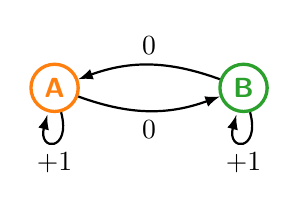
\begin{tikzpicture}
\tikzstyle{n} = [very thick,circle,inner sep=0mm,minimum width=6mm]
\tikzstyle{a} = [thick,>=latex,->]
\def\dx{1.2}
\def\dy{-1.2}
\node[n,C1,draw=C1] (2) at (\dy,0) {\textbf{\textsf{A}}};
\node[n,C2,draw=C2] (1) at (\dx,0) {\textbf{\textsf{B}}};
\path[a]
(2) edge [loop below] node {+1}(2)
(1) edge [loop below] node {+1}(1)
(2) edge [bend right=20] node[below] {0}(1)
(1) edge [bend right=20] node[above] {0}(2);
\end{tikzpicture}

The reinforcement learning agent performs Q-learning.  Recall the $Q$ table has entries $Q(s,a)$.
The $Q$ table is initialized with all zeros.
The agent starts in state $s_1=A$.
In any state $s_t$, the agent chooses the action $a_t$ according to a behavior policy $a_t = \pi_B(s_t)$.
Upon experiencing the next state and reward $s_{t+1}, r_t$ the update is:
$$Q(s_t, a_t) \Leftarrow (1-\alpha) Q(s_t, a_t) + \alpha \left( r_t + \gamma \max_{a'} Q(s_{t+1}, a') \right).$$
Let the step size parameter $\alpha=0.5$.

\begin{enumerate}
\item Run Q-learning for 200 steps with a uniformly random behavior policy: $\pi_B(s_t)=$ move or stay with 1/2 probability for any $s_t$.
Show the Q table at the end.

\begin{soln}

\begin{center}
\begin{tabular}{c|ccc}
& A & B \\\hline
Stay&9.234484015623739&9.121017499190112&\\
Move&8.20613430968956&8.19636873756536&
\end{tabular}
\end{center}
	
\end{soln}

\item Reset and repeat the above, but with an $\epsilon$-greedy behavior policy: at each state $s_t$, with probability $1-\epsilon$ choose what the current Q table says is the best action: $\argmax_a Q(s_t,a)$; Break ties arbitrarily. Otherwise (with probability $\epsilon$) uniformly chooses between move and stay.
Use $\epsilon=0.5$.


\begin{soln}

\begin{center}
\begin{tabular}{c|ccc}
& A & B \\\hline
Stay&9.104247838429991&9.977658669697917&\\
Move&8.968218232479222&8.072212822570261&
\end{tabular}
\end{center}
	
\end{soln}


\item Reset and repeat the above, but with a deterministic greedy behavior policy: at each state $s_t$ use the best action $a_t \in \argmax_a Q(s_t,a)$ indicated by the current Q table. If there is a tie, prefer move.

\begin{soln}

\begin{center}
\begin{tabular}{c|ccc}
& A & B \\\hline
Stay&0.0&0.0&\\
Move&0.0&0.0&
\end{tabular}
\end{center}
	
\end{soln}

\item Without doing simulation, use Bellman equation to derive the true Q table induced by the MDP.

\begin{soln}
\\Bellman's Equation for Q learning: $Q(s,a) = r(s,a) + \gamma \max_{a'}Q(s',a')$ where state = s, and action = a

When state is A and stay, using the equation above,
\\Q(A,stay) = r(A,stay) + $\gamma$*max(Q(A,stay),Q(A,move)) 
\\As Q(A,stay) = 0, Q(A,move) = 0 and r(stay) = 1
\\Therefore, Q(A,stay) =   1 + 0.9(0) = 1 

For next updation, Q(A,stay) = 1 + 0.9(1)
\\So after updations, Q(A,stay) = $1 + 0.9 + 0.9^2 + 0.9^3 ... = \frac{1}{1-0.9} = 10$

When state is B and stay, similar to the above,
\\Q(B,stay) = $1 + 0.9 + 0.9^2 + 0.9^3 ... = \frac{1}{1-0.9} = 10$
 
When state is B and move,
\\Q(B,move) = r(B,move) + $\gamma$ max(Q(A,stay),Q(A,move)) = 0 + 0.9*Q(A,stay) = 0.9*10 = 9

When state is A and move,
\\Q(A,move) = r(A,move) + $\gamma$ max(Q(B,stay),Q(B,move)) = 0 + 0.9*Q(B,stay) = 0.9*10 = 9
	
Q table is given below,
	
\begin{center}
\begin{tabular}{c|ccc}
& A & B \\\hline
Stay&10&10&\\
Move&9&9&
\end{tabular}
\end{center}

\end{soln}


\end{enumerate}


\end{document}
